\chapter{Introduction}

Anomaly detection is an important task in environments where we have a good knowledge of what is the normal behaviour but we know very little about the behaviour of anomalies. The reasons for this can be numerous: either there is no common generating principle behind the anomalies, or there is a huge disbalance in the number of labeled normal and anomalous data samples that are available for us (sometimes no anomalies are available at all), or the acquisition of anomalous data is too expensive or downright impossible (an example of this might be an industrial process). While it might be tempting to solve anomaly detection as supervised binary classification, for the reasons listed above, a supervised classificator is likely to be unrobust to actual anomalies that it will encounter in a production environment. Together with an ever-increasing volume of collected data and available computing power, this motivates the development of specialized methods for automatic anomaly detection. What these methods have in common is that they learn a model of normal data in an unsupervised manner, and detect anomalies as deviations from this model. 

Anomaly detection is important for many industries, where it is typically difficult to obtain a representative training set containing representative samples of anomalous data. The actions taken after an anomaly is detected might be varied. Sometimes, the anomaly might be considered to be an erroneous measurement and as such is ignored, which is the case of some of the earliest scientific essays~\cite{glaisher1873rejection,edgeworth1887xli} on the topic of anomaly detection. In other cases, a preventive measure must be taken in order to mitigate unwanted behaviour, such as the case of cybersecurity~\cite{liao2013intrusion, vanerio2017ensemble,xin2018machine}, fraud detection~\cite{bolton2002statistical, perols2011financial, ahmed2016survey}, medical diagnosis~\cite{tarassenko1995novelty, wong2003bayesian, iakovidis2018detecting,zhou2019anomalynet} or industrial process monitoring~\cite{mahmoudi2019layerwise, bai2020anomaly, choi2020gan}. Finally, detected anomalies might drive forward scientific discovery in astronomy~\cite{protopapas2006finding}, plasma physics~\cite{vskvara2020detection}, chemistry~\cite{oprea2002chemical} or particle physics~\cite{fraser2022challenges}.

There are countless models and algorithms for anomaly detection, tackling the problem from different angles based on the basic principle of the algorithm, the expected nature of the data and application domain. There are methods based on random forests\,\cite{liu2008isolation}, the k--nearest neighbors algorithm\,\cite{harmeling2006outliers}, Gaussian mixture models\,\cite{mahadevan2010anomaly}, clustering neural networks\,\cite{schlegl2017unsupervised}, histogram estimation\,\cite{pevny2016loda}, kernel density estimates\,\cite{latecki2007outlier} or support vector machines\,\cite{scholkopf2001estimating}. A comprehensive overview of anomaly detection methods is presented in studies such as\,\cite{pimentel2014review,goldstein2016comparative,lazarevic2003comparative,chandola2009anomaly,campos2016evaluation} where the authors compare several existing methods on benchmark datasets. Most of the comparative studies however do not include methods based
on (deep) neural networks and especially not generative models. The probably most recent and complete overview of deep generative models can be found at~\cite{ruff2020unifying}.

Deep generative models have recently attracted a lot of attention due to their ability to produce (generate) very high quality artificial images that resemble those from he training dataset. Since the seminal papers\,\cite{goodfellow2014gan,kingma2013vae,dinh2014nice} on the main types of generative models have been published, a myriad of improvements and tweaks have been proposed. While the original purpose of generative models was not aimed towards anomaly detection, some of them were redesigned for it. This text intends to collect some (but definitely not all) of the relevant information on deep generative models in one place and assess the potential suitability of the different generative models to the task of anomaly detection.

This chapter is organized in the following fashion: first, the basic principles of anomaly detection are introduced. Then we follow with a classification of anomaly detectors into main categories based on their principles and their short description, as it will be useful in the later chapters. A short section on the evaluation of anomaly detectors is followed by an overview of datasets that are frequently (and in this text) used for their experimental comparison and demonstration of their capabilities.

\section{What is anomaly detection?}

\note{
Here, use an example of an anomaly detection problem.

Define P as normal distribution.

Solo/contextual (semantic)/group anomalies.
}

Anomaly detection has been extensively studied under many different names: outlier detection~\cite{knorr98algorithms,hodge2004survey}, novelty detection~\cite{pimentel2014review}, one-class classification~\cite{ruff2018deep} or out-of-distribution detection~\cite{liang2017enhancing}. There is a small distinction between the terms outlier, novelty and anomaly, although often times the terms are used interchangeably. The methods for their detection are however usually based on the same principle, therefore, we will resort to the use of the last term. An often cited definition of what constitutes an anomaly is ``an observation which deviates so much from other observations as to arouse suspicion that it was generated by a different mechanism''~\cite{barnett1974outliers}. This broad statement highlights the fact that anomalies may have very different sources of origin and them being anomalous depends on the context in which they are considered. 

The probabilistic definition assumes a probability distribution $P^+$ of normal data, operating on a data space $\mathcal{X}$, which is defined by a given problem, and which is most of the time known only through a set of normal samples. We can call a sample $x \in \mathcal{X}$ anomalous if it lies in a region where $P^+$ has very low density. In other words, we can define a set of anomalies~\cite{ruff2020unifying} as 
\begin{equation} \label{eq:anomaly_set}
	\mathcal{A} = \lbrace x \in \mathcal{X} \vert p^+(x) \leq \tau \rbrace, \tau \geq 0,
\end{equation}
where $p^+(x)$ is the probability density function corresponding to $P^+$ and $\tau$ is a threshold which defines the line between normal and anomalous samples. 

It is also often assumed that the region of data space that is occupied by normal data is concentrated, that is, there exists a threshold $\tau \geq 0$ such that
\begin{equation} \label{eq:anomaly_set}
	\mathcal{X} \slash \mathcal{A} = \lbrace x \in \mathcal{X} \vert p^+(x) > \tau \rbrace
\end{equation}
is not empty, which however does not imply that the support of $p^+$ is bounded. On the other hand, $\mathcal{A}$ is not required to be concentrated and can be unbounded. Notice that we do not explicitly define any sort of anomalous distribution $P^-$. This is because most anomaly detection methods only model $P^+$. When $P^-$ is considered, such as in KDE~\cite{parzen1962estimation} or OCSVM~\cite{scholkopf2001estimating}, it is assumed that it is uniform over $\mathcal{X}$. 

Different types of anomalies which require different approaches have been identified in literature~\cite{chandola2009anomaly,ruff2020unifying}. 
\begin{itemize}
	\item[Point anomaly] is a single datapoint of $\mathcal{A}$, for example an outlying measurement or a photograph of a cat among other images of dogs. This is the most often studied type of anomaly in research literature.

	\item[Contextual] anomaly is a kind of anomaly that is only anomalous in certain context. A person measuring over 195~cm might be an outlier in almost any place save for a locker room of a basketball team. If a target dataset consists of pictures of birds photographed mid-flight -- is a bird sitting on grass an anomaly? Or a different flying object, such as an airplane? The answers to those questions depends on what problem is actually being solved. Contextual anomalies often arise in time series~\cite{tsay2000outliers} or in spatial data~\cite{chawla2006slom}.

	\item[Group anomalies] are a collection of correlated datapoints that are only anomalous together. Only a large number of malicious requests is enough to shut down a server in a DDoS atack~\cite{ahmed2018collective}. Other research~\cite{quellec2016multiple,wan2020weakly} focuses on finding anomalies under the multiple-instance learning (MIL)~\cite{carbonneau2018multiple} paradigm, where individual datapoints (called bags) are comprised of a variable number of observations or measurements (called instances). This calls for an aggregation method, on top of which an anomaly detector can operate.

	\item[Semantic] anomalies arise in image data and are opposed to \textbf{sensory} anomalies. While sensory anomalies appear in low-level image features such as edges or textures (e.g. breaks or defects), semantic anomalies can be detected in the high-level information of an image (e.g. an object of a different category than what appears in the  training dataset). Semantic anomalies can be hard to detect, as they can be very similar to normal data~\cite{ahmed2020detecting}. We will cover their detection in chapters~\ref{sec:chapter_comparison} and~\ref{sec:chapter_sgvaegan}.
\end{itemize}

\subsection{Anomaly score}
We can think of any anomaly detection model as providing a function that produces ranking of the individual data points with respect to their anomalousness. This is called an \textbf{anomaly score function} $s:\mathcal{X}\rightarrow\mathbb{R}$ of a model. An \textbf{anomaly score} of a datapoint $x$ is the number $s(x)$. In certain contexts~\cite{pedregosa2011scikit}, anomaly score function might be called \textit{decision }or \textit{scoring function}. In this text we will assume that a higher anomaly score is attributed to a point more likely to be anomalous. As is evident from the definition, the anomaly score function does not need to be a probability in the sense of its function values lying in the interval $\left[0,1\right]$ -- in fact, some models can produce negative anomaly scores. To be able to use an anomaly score function for decision making, one must choose threshold $\tau\in\mathbb{R}$. From~\eqref{eq:anomaly_set}, a sample $x$ is considered to be an anomaly if $s(x)>=\tau$ and normal otherwise. The selection of $\tau$ can sometimes be a process more complicated than the fitting


of the actual model. Finally, we define the \textbf{contamination rate} of a dataset $X$, which is a finite collection of samples from $\mathcal{X}$ as
\begin{equation}
C(\mathcal{X})=\frac{|\{x_{i}|x_{i}\in \mathcal{A} \wedge x_i \in X \}|}{|\{x_{i}|x_{i}\in X\}|},
\end{equation}
i.e. the ratio of the number of anomalies to the total size of the dataset.


\section{Metrics for anomaly detector comparison}

However the authors never ask the question if the way the methods are compared to each other is appropriate for the anomaly detection setting. The area under receiver operating characteristic curve (ROC AUC or just AUC in this text) seems to be the gold-standard of the field, as it allows to compare models by a single number. In \cite{vanderlooy2008critical}, the authors compare "soft" variants of AUC in which the contribution of a sample to the total value of AUC is weighted by the degree in which it is labeled correctly or incorrectly. They demonstrate that none of these alternatives can systematically outperform the conventional AUC, however they do so on a set of binary classification experiments, without any consideration for the specifics of anomaly detection.


While AUC is a darling performance measure of anomaly detection of researchers, practitioners rely on other measures better reflecting their needs. For example in intrusion detection, precision@k is popular \cite{grill2016learning}, since the security officer can investigate at most $k$-most anomalous samples a day and he wishes to find as many dangerous security incidents present in the data as possible. Similarly, the true positive rate at a fixed false positive rate is used in tuning anti-virus engines, as these applications need to be certain not to raise too many alarms to the users (discussions with experts from the field suggests the tolerable false positive rate to be in order $10^{-4}$). Other security application domains, fraud detection, control of industrial and environmental processes, and others have similar application constraints emphasizing low false positive rates. We believe not to exaggerate if we state that for the purpose of anomaly detection, the region of low false positive rates in the ROC curve might be the most critical for evaluating the performance of a method. 

Imagine now a data-scientist developing new anomaly detection tools supporting the above applications. They wish to implement a state of the art algorithm, which can represent a significant time investment, yet all papers available to them compare the proposed detectors using AUC. How does AUC help them to decide which method to implement, if he is interested in performance measured by precision@k? AUC may be misleading since it is an integral over all possible thresholds, putting equal emphasis on each threshold, where most of them are far off his point of interest. How much are they certain that the proposed detector is not degenerated, as is shown in Figure~\ref{fig:bad_auc}?

We admit that other measures than AUC are sometimes reported. In \cite{mahadevan2010anomaly}, equal error rate is reported together with AUC. In \cite{lazarevic2003comparative}, detection rate is used to compare methods. In the anomaly detection survey \cite{campos2016evaluation}, average precision and precision@k adjusted for class imbalance are reported together with AUC and it is concluded that their behaviour is very dataset-dependent and less stable than that of AUC, but no deeper insight is given.

In this paper the subject of interest are performance measures instead of anomaly detection algorithms themselves. Our goal is to shed more light on behavior of different measures. Particularly we want to quantify how different measures are correlated with each other and what happens if a detector is selected using a different measure than the one that is used in the application. Our endeavor is to suggest an alternative measure which would be more descriptive of the performance for practitioners. 

While the problem of choosing the right measure seems to be solvable using some variants of AUC, we also demonstrate a more profound problem: if the validation set contains examples of anomalies with different statistical properties (probability distributions) than anomalies in the testing set, the performance measures are not informative. The only exception is the volume of decision region, which does not rely on anomalous samples and is theoretically justified \cite{steinwart2005classification}. Unfortunately, the volume of decision region is difficult to estimate in higher dimensions.

The original scenario in which the receiver operating characteristic (ROC) curve \cite{egan1975signal} and the corresponding area under the curve (AUC) was used as a performance measure is binary classification, which is closest to supervised anomaly detection setting. However, it is commonly used for evaluation in all of the three separate settings without any hesitation, even though there is no real second class in the semi- and unsupervised cases. The typical argument justifying its use is that the precise application conditions enabling to measure detection accuracy at a precise false positive rate are unknown, therefore AUC offers a good solution as it summarizes all application conditions. While this is true, it also means that these other application conditions are very different from those of our interest, which possibly negatively influences our decision. 

We assume that for an input $x$ an anomaly detection algorithm produces a real-valued anomaly score instead of a binary value, i.e. it is a projection $f:\mathcal{X} \rightarrow \mathbb{R}$ from the sample space $\mathcal{X}$. We also assume that higher score corresponds to samples more likely to be anomalous. Anomaly score does not have to be a probability in the range $[0, 1]$ or even a positive number (e.g. in the OC-SVM model). 

When a sample is to be labeled as normal / anomalous, the output of the detector is compared to a threshold. Its value is typically determined on basis of tolerated false positive rate and an estimate of the true contamination rate of a dataset $X$, which we define as $C(X)=\frac{P}{P+N}$, where $P$ and $N$ is the total number of positive and negative samples in $X$.

\begin{table}
\centering
	\begin{tabular}{c | c c}
		true label/estimated label & normal & anomalous \\
		\hline
		normal & tn & fp  \\
		anomalous & fn & tp 
	\end{tabular}
	\caption{A confusion matrix of a model.}
	\label{tab:conf_ex}
\end{table}

Table~\ref{tab:conf_ex} displays the confusion table that introduces basic concepts and notation needed below. It summarizes the performance of an algorithm with a particular threshold by presenting the total number of correctly (tp = true positives and tn = true negative) and incorrectly (fp = false positives and fn = false negatives) identified samples. 


\subsection{Area under the ROC curve}
The most widely used measure in the field of anomaly detection is the area under the ROC curve (the acronym AUC will be used in the following text for the sake of brevity). The ROC curve is a parametric curve describing the trade-off between true positive rate $\text{TPR}(\tau) = \frac{\text{tp}}{\text{tp+fn}}(\tau)$ and false positive rate $\text{FPR}(\tau) = \frac{\text{fp}}{\text{fp+tn}}(\tau)$ for different values of the decision threshold $\tau$. A ROC curve can be easily computed on a dataset from the knowledge of the true labels and anomaly scores of the samples. 

Then, the area under the curve is calculated as the following integral
\begin{equation}
\label{eq:auc}
\text{AUC}=\int_{\mathbb{R}}\text{TPR}(\tau)d\text{FPR}^{\prime}(\tau)d\tau = \int_0^1\text{TPR}(\text{FPR})d\text{FPR}.
\end{equation}
The last integral that uses $\text{TPR}(\cdot)$ as a function of the corresponding FPR shows the simple concept behind the AUC that can be easily discerned from a ROC curve drawn in a graph. An example of a ROC curve and the corresponding AUC is in Figure \ref{fig:ROC}. In practice, the corresponding AUC is estimated from an empirical ROC curve using some numerical integration scheme, e.g. the trapezoidal rule.

As mentioned above, the main advantage of AUC is that it does not depend on the choice of a particular decision threshold. Also, the measure has a straightforward interpretation -- it is an estimate of the probability that a randomly chosen positive sample is ranked higher than a randomly chosen negative sample \cite{hand2001simple}. However a lot of information is lost when the whole ROC curve is summarized into a single number. This is especially concerning for the case of anomaly detection, where usually the region of low false positive rates is of interest, since anomalies are sparse with respect to normal data and we strive to achieve a low false positive rate. It is frequent in security applications to draw ROC curve with a logarithmic scale on the x-axis.

\begin{figure}
\centering
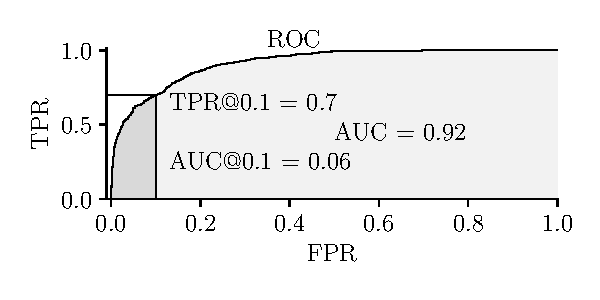
\includegraphics[scale=0.85]{data/chapter_intro/fig_roc.pdf}
\caption{An example of ROC curve and the derived measures based on FPR=0.1. AUC is the whole shaded area under the ROC curve. The darker shading corresponds to AUC@0.1.}
\label{fig:ROC}
\end{figure}

\subsection{\auca}
A simple alternative to AUC is calculated only up to some value of false positive rate $\alpha$. Numerically, it is important to interpolate the ROC curve for a given $\alpha$ before computing the integral, especially for datasets with a small number of samples. In illustration on Figure~\ref{fig:ROC}, AUC@0.1 corresponds to the darker gray region. \auca\ can be easily normalized by dividing by the chosen $\alpha$, in which case the best detector has $\auca = 1$ similarly to AUC.

\subsection{\tpra}
Another performance measure popular among practitioners (anti-virus engine vendors) is simply the true positive rate (TPR) evaluated at a given false positive rate (FPR) $\alpha.$ This measure can be easily read from a ROC curve, and as in the case of \auca, in practice it is necessary to interpolate the ROC curve since FPR has discrete values.

\subsection{Weighted AUC}
\tpra~belongs to a class of Neyman Pearson measures \cite{scott2007performance}, where the goal is to find a classifier minimizing error of one type while the error of the other is bound by some value. It has been shown in \cite{scott2007performance}, that for a given bound on the false positive rate $\alpha$, the best classifier $f$ from a class of classifiers $\mathcal{F}$ consistently minimizing the true positive rate can be found as
\begin{equation}
\arg \min_{f\in\mathcal{F}} \frac{1}{\alpha} \max\{\text{FPR}(f) - \alpha, 0\} + (1 - \text{TPR}(f)),
\end{equation}   
where $\text{FPR}(\cdot)$ and $\text{TPR}(\cdot)$ denotes the false and true positive rate of a particular classifier.

This puts more weight on the region of low FPR values proportionate to $1/\text{FPR}(\alpha)$. In a manner similar to the definition of AUC~\eqref{eq:auc}, we can define the weighted AUC as an integral over all values $\alpha$ as
\begin{equation}
\aucw=\int_0^1\text{TPR}(\text{FPR})\text{FPR}^{-1}d\text{FPR},
\label{eq:AUCw}
\end{equation}
where we define $\text{FPR} = 0$ as $\text{TPR}(\text{FPR})\text{FPR}^{-1} = 0$, which makes the integral proper. While it might seem that this definition may still result in an arbitrary large number, in practice, the FPR in the ROC curve changes by a given finite increment that equals $1/p$, where $p$ is the total number of positive samples. This means that \aucw~attains comparable values, although it is not easily normalized like the remaining measures described here, which might create some issues in the former analysis.

Figure \ref{fig:AUCw} illustrates the motivation behind \aucw~showing ROC curves of two detectors. First detector with the ROC curve drawn with solid has a higher AUC than the second detector with ROC curve drawn in dashed line. If we base the selection on AUC, we would choose the first detector. Yet, this detector has inferior performance in the area of low false positive rate, where the second is better. If the decision would be based on the \aucw, the second detector would be selected. 

\begin{figure}
\centering
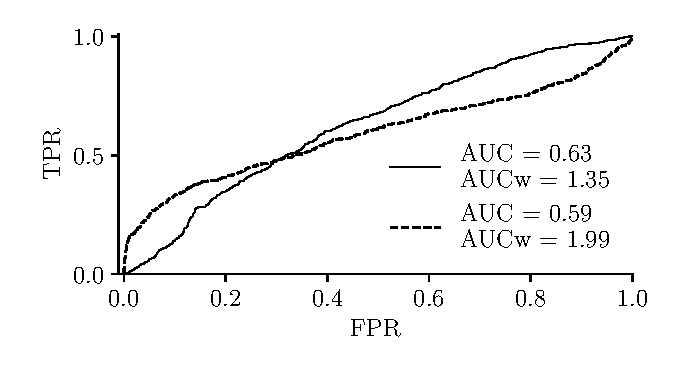
\includegraphics[scale=0.85]{data/chapter_intro/fig_auc_weighted.pdf}
\caption{Two ROC curves with different AUC and \aucw.}
\label{fig:AUCw}
\end{figure}

\subsection{\preca} \label{preca}
In binary classification, the precision, given a real--valued threshold $\tau$, is defined as $\text{PREC}(\tau)=\frac{\text{tp}}{\text{tp + fp}}(\tau)$. To make this measure more appropriate for anomaly detection setting, only $p\%$ most anomalous samples can be taken into account. Unfortunately, this measure is difficult to compare across datasets, because it depends on the proportion of anomalies with respect to normal samples. To make the measure comparable, the definition has been adapted as follows. First, anomalies are randomly removed from the testing dataset on which we want to evaluate the detector such that their proportion is $p$\%. This sub-sampled testing dataset is denoted $X$, and the \preca~is calculated as follows
\begin{equation}
  \text{Precision@}p = \frac{|\lbrace x \in X_p \land \text{ true label of } x \text{ is positive}  \rbrace|}{|X_p|},
\end{equation}
where $X_p$ is the set of $p\%$ most anomalous samples in $X$. With a perfect detector, $X_p$ should contain all the anomalies and nothing else, thus yielding \preca = 1.

\subsection{Volume of decision region}
\begin{figure}
\centering
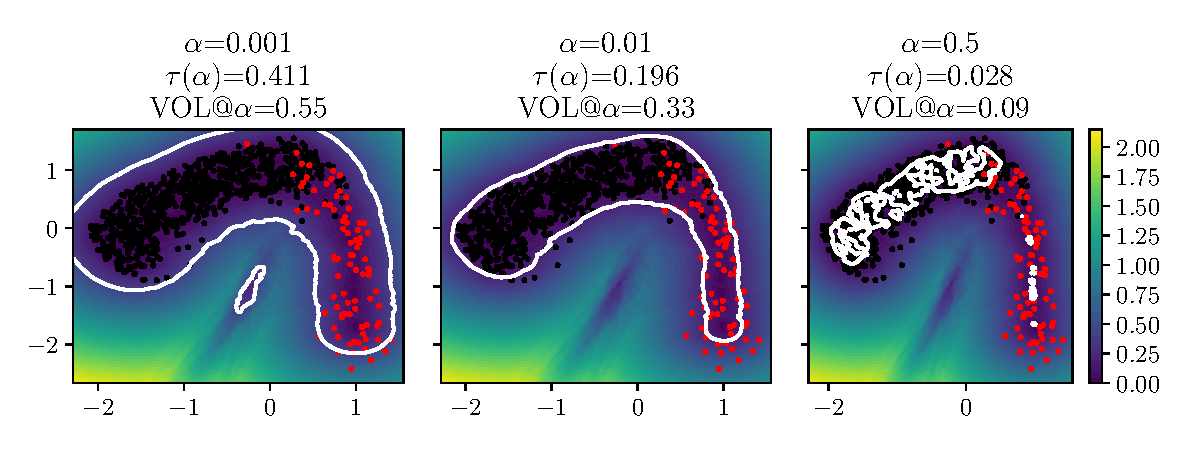
\includegraphics[scale=0.8]{data/chapter_intro/fig_vol_example.pdf}
\caption{An example of a detector and the decision region for differing values of FPR $\alpha$. The decision boundary is drawn as a white isoline at level $\tau(\alpha)$ with the estimated enclosed volume $\text{VOL@}\alpha$, black and red dots represent normal and anomalous samples in the training set. Clearly, smaller tolerance of false positives forces us to set a higher threshold which results in higher decision region volume.}
\label{fig:vol_example}
\end{figure}
All of the previous measures originate from evaluation of performance of binary detectors. Since semi- and unsupervised anomaly detection is closer to one-class classification or density estimation, a measure that does not require labels for its evaluation might be more useful and better describe behaviour on unknown samples. If the goal is to compare two models supposed to characterize the normal class, it makes sense to choose the model enclosing the training data more tightly. This corresponds to calculating  the volume inside the model's decision boundary in a similar fashion to \cite{clemenccon2013scoring}, where a theoretical justification is given. This decision boundary can be chosen to correspond to a certain level of false positive rate. We define the volume of decision region as
\begin{equation}
  \text{VOL}(\alpha) = \int_{\mathcal{X}} \mathds{1}_{\lbrace x\in\mathcal{X}|f(x) <= \tau\rbrace} \left( x \right) dx  \text{ s.t. } \text{FPR}(\tau)=\alpha,
\end{equation}
where $\mathcal{X}$ is the input space, $f(x)$ is a decision function, $\tau$ is the decision boundary (threshold) and $\alpha$ is a given false positive rate. In other words, $\text{VOL}(\alpha)$ is the volume of subset of input space where classifier returns "normal" answer. An example of a model and its decision region for different values of $\alpha$ is shown in Fig.~\ref{fig:vol_example}. It should be noted that the idea of minizing the enclosed volume is native to some models, e.g. the OC-SVM algorithm \cite{scholkopf2001estimating}.

\begin{algorithm}
    \caption{Volume of decision region computation}
    \label{alg:vol}
    \begin{algorithmic}[1]
    \Require{FPR $\alpha \in \left[0,1\right]$, a set of samples $X=\lbrace x_i \rbrace \in\mathbb{R}^d$, vector of true labels $y=\lbrace y_i\rbrace$, vector of anomaly scores $a=\lbrace a_i\rbrace$, number of samples $N \in \mathbb{N}$, a decision function $f(x)$}
    \State{$\text{TPR},\text{FPR} \gets$ Compute the ROC curve from $y$ and $a$.}
    \State{$\tau \gets$ Interpolate the ROC curve using $\alpha$ to estimate the corresponding decision threshold}
    \State$b_{min} \gets \left\{ \min_{i}(x_{ij}),j\in\hat{d}\right\}$ lower sampling boundaries
    \State$b_{max} \gets \left\{ \max_{i}(x_{ij}),j\in\hat{d}\right\}$ upper sampling boundaries
    \State{$k \gets 0$} Normal samples counter
    \For{$n\in\lbrace1,2,\dots,N\rbrace$}
      \State{$x \gets $ Sample drawn from uniform distribution $\mathcal{U}(b_{min}$,$b_{max})$}
      \State{$a_x \gets f(x)$ anomaly score of $x$}
      \If{$a_x<\tau$}
        \State{$k \gets k+1$}
      \EndIf
    \EndFor
    \State{\textbf{return} $\text{VOL@}\alpha=\frac{k}{N}$}
    \end{algorithmic}
\end{algorithm}

Computing the empirical $\text{VOL}(\alpha)$ in data space $\mathcal{X}$ is difficult and is numerically estimated by Monte-Carlo methods. In this work, we have adopted the algorithm as described in Alg. \ref{alg:vol}. From the definition, it is clear that the empirical measure is already normalized any can be compared across models as long as the input set of samples $X$ or the sampling boundaries are kept fixed. A preferable model yields a lower \vola. Therefore the search for an optimal model is a minimization problem. This is in contrast with the measures that were described above, which are always maximized. To make the further analysis simpler, we define the complementary normalized volume outside of the decision boundary
  \begin{equation}
    \cvola = 1-\vola
  \end{equation}

The main issue with VOL@$\alpha$ is the computational cost. Firstly, the number of samples required to cover $r$--dimensional sample space grows exponentially with $r$. Secondly, it requires $N$ evaluations of the anomaly score, which might be prohibitively expensive for some models. The first issue has been adressed in \cite{goix2016evaluate}, where the volume is computed multiple times for different subsampling of input features, however this does not seem to be optimal as it requires training a new model for each subset of features, therefore it has not been done in this paper.

\subsection{Other measures}
There are other measures that are sometimes considered for evaluation of anomaly detection models. Here we will shortly mention two of them and give reasoning for why they were not included in the experimental analysis.

\textbf{AUPRC}, or Area Under the Precision--Recall Curve, is given by computing precision (see the definition in \ref{preca}) and recall $\text{REC}(\tau) = \frac{\text{tp}}{\text{p}}(\tau)$ for different values of classification threshold $\tau$ and then integrating the area under the resulting curve. A PR curve has at most as many unique recall values as positive samples in the dataset. This is problematic for anomaly detection, where the number of anomalies is low, which leads to a very sparse estimate of the true PR curve. Also, our experiments make extensive comparison across different datasets with varying amount of anomalies, to which a PR curve is very sensitive. In fact, using the same trained anomaly detector and changing the contamination rate of a testing dataset produces different AUPRC results, which then makes any analysis based on AUPRC useless when the true contamination rate is unknown. Furthermore, a correct PR curve lacks a universal starting point unlike ROC, because precision is undefined for zero recall, making the computation and normalization of the area under the PR curve and the comparison between datasets even more complicated. Further critique of AUPRC compared to ROC--based measures do not have are described in \cite{flach2015precision} -- there is no universal baseline given by a completely random detector, PR curves cannot be interpolated, the AUPRC has no other than geometric meaning etc. Finally, it has been shown \cite{davis2006relationship} that PR and ROC curves contain the same points. Therefore we ommit AUPRC from our experiments.

% http://pages.cs.wisc.edu/~boyd/aucpr_final.pdf claims that PR curve -> (0,1) if highest score is a positive sample and -> (0,0) if it is not

\textbf{F1--score} is a single number computed as $\text{F}_1(\tau) = \frac{\text{2tp}}{\text{2tp+fp+fn}}(\tau)$ \cite{chinchor1992muc}. It was designed for unbalanced datasets as it is a harmonic mean of precision and recall. However, the same issues arise for comparison between datasets containing a different number of anomalies. Also, F1--score puts equal weight on precision and recall. This is however in direct contrast with common practice in anomaly detection, where the focus is usually only on one of these.

\section{Anomaly detectors taxonomy}

This section follows the taxonomy outlined in~\cite{pimentel2014review, ruff2020unifying}.


\subsection{Probabilistic}

Mahalabonis, GMM, DAGMM, ARIMA, extreme values, HMM, Loda, HBOS, KDE

EBMs, Flows

\textbf{Gaussian mixture models} in\,\cite{mahadevan2010anomaly}


The \textbf{lightweight on--line detector of anomalies} (Loda)\,\cite{pevny2016loda}
algorithm is based on an ensemble of one--dimensional histograms
in a space of diversified projection vectors. The anomaly score is
then an average of the logarithm of probabilities estimated from the
histograms on individual projection vectors. Due to its simplicity
and computational efficiency, it is popular in settings with high
volumes of data and potentially missing input values.


\subsection{Domain-based/Classification}

OCSVM, SVDD, HSC

GT, GDAD, DSVDD, OCNN, Discriminator

One of the more popular models is the \textbf{one-class SVM} (OCSVM)\,\cite{scholkopf2001estimating}
which estimates the support of the normal (non--anomalous) data with
the use of non--linear kernel functions.

\subsection{One Class Support Vector Machines (OC-SVM)}
OC-SVM \cite{scholkopf2001estimating} estimates the support of the training data distribution to be able to decide whether an unlabeled sample belongs to it or not. It uses a non-linear kernel function to compute the projection from the original input space to a feature space of higher dimension, in which it is possible to linearly separate the bulk of the training data by a hyperplane. The anomaly score is then the signed distance of a point from the hyperplane.  The RBF kernel will be used and the inverse of the width of the kernel $\gamma$ will be tuned. In our experiments, the hyperparametr $\nu$, which acts as an upper bound on the number of anomalies in training data, will not be tuned and will have the value 0.5 as we believe that the value of $\gamma$ is more critical to the performance.


\subsection{Distance-based}

kNN, HighDoD, LOF, LOCI, k-means?, ABOD, IF, 

One of the simplest models is the \textbf{kNN} model for
unsupervised anomaly detection where the anomaly score of a sample
is its proximity to its k--nearest samples. Several definitions of
different proximity measures are described in\,\cite{harmeling2006outliers}.
Despite its simplicity, it has been shown e.g. in\,\cite{campos2016evaluation}
that it is one of the most universal unsupervised models.

\subsection{k-Nearest Neighbours (kNN)}
The kNN algorithm \cite{ramaswamy2000efficient} is a simple but efficient model. A measure of anomalousness is the distance of a sample $x$ to its $k$-nearest neighbours. In this paper, three different ways to compute the kNN anomaly score are going to be used in accordance with \cite{harmeling2006outliers}. These are sometimes treated as different algorithms, however we are going to treat them as hyperparameters.
\begin{itemize}
  \item $\kappa(x)$: the anomaly score is the distance between $x$ and its $k$th-nearest neighbor.
  \item $\gamma(x)$: the anomaly score is the average distance of $x$ to its $k$-nearest neighbors. 
  \item $\delta(x)$: the anomaly score is the length of the mean of the vectors pointing from $x$ to its $k$-nearest neighbours.
\end{itemize}



\subsection{Local Outlier Factor (LOF)}
The LOF algorithm \cite{breunig2000lof} is based on comparing the local density of a sample $x$ with the local density of its $k$--nearest neighbours. To correctly describe the way in which the density is defined and the anomaly score is computed, let's define $k$-distance $k\text{-dist}(x)=\max_{y \in N_k(x)} d(x,y)$, where $N_k(x)$ is the set of the $k$--nearest neighbours (which can, in this context, actually contain more than k samples if some are tied at the $k$-dist$(x)$) of $x$. Also, $d(x,y)$ is the distance between $x$ and $y$ (e.g. Euclidean distance). Then we can define reachability distance $\text{rd}_k(x,y)$ as $$\text{rd}_k(x,y)=\max \lbrace k\text{-dist}(y), d(x,y) \rbrace.$$ This formula can be used to define the \textit{local reachability density} as 
\begin{equation}
  \text{LRD}_k(x)=\frac{|N_k(x)|}{\sum_{y\in N_k(x)}\text{rd}_k(x,y)}.
\end{equation}
It is in fact the inverse of average reachability--distance of $x$ and its neighbours. Finally, anomaly score of $x$ is given by comparing the $\text{LRD}_k(.)$ of $x$ and its neighbours 
\begin{equation}
  \text{LOF}_k(x)=\frac{\sum_{y\in N_k(x)} \text{LRD}_k(y)}{\text{LRD}_k(x) |N_k(x)|}.
\end{equation}




A different way of local density estimation is used in the \textbf{local
outlier factor} (LOF) algorithm\,\cite{breunig2000lof}, which is
based on comparing the local density of a sample with local densities
of its k--nearest neighbors. Similar methods are the \textbf{connectivity--based
outlier factor} (COF)\,\cite{tang2002enhancing} or \textbf{clustering--based
local outlier factor} (CBLOF)\,\cite{he2003discovering}.

A different approach is taken by the \textbf{isolation forest }(IF)
model\,\cite{liu2008isolation} where a forest of isolation trees
is constructed for the whole dataset. Isolation trees are constructed
in such a way as to isolate each individual datapoint from the rest
of the dataset using consecutive splits on different features. It
is presumed that an anomaly can be isolated using a smaller number
of splits and therefore it lies on a branch closer to the root of
the tree. The anomaly score is then the number of splits of a sample
averaged over multiple randomly initialized trees in the ensemble.

\subsection{Isolation Forest (IF)}
Isolation Forest \cite{liu2008isolation} is an algorithm based on random forests. During training, the input space is recursively and randomly cut into multidimensional boxes so that all training data points are isolated. A single cut can be expressed in terms of a tree structure with data points on the tips of the branches. An Isolation Forest instance consists of a number of such trees. It can be shown that anomalies usually require less cuts to be isolated -- in other words they are more likely to be on branches that are shorter. Therefore, an anomaly score is computed from the average path length from the root of the tree to the datapoint. The hyperparameter to be optimized is the number of trees $N_t$.

\subsection{Reconstruction-based}

PCA, vQ, Kmeans?, 

AE, CAEs, DAEs, VAEs, Generator

Methods based on the \textbf{PCA }transformation\,\cite{shyu2003novel,aggarwal2015outlier}\textbf{
}are also available for anomaly detection. It is presumed that normal
data lie on a lower dimensional manifold in the data space which is
extracted by selecting the covariance matrix eigenvectors with highest
corresponding eigenvalues. The distance to this manifold is then used
as anomaly score.


\begin{figure}
\begin{centering}
\begin{tikzpicture}
  \node[const]                               (x) {$\vc{x}$};
  \node[const, right = 0.5cm of x]           (xin) {};
  % encoder in
  \node[latent, right = 0.6cm of x, yshift = 0.825cm] (E11) {};
  \node[latent, right = 0.6cm of x, yshift = 0.275cm] (E12) {};
  \node[latent, right = 0.6cm of x, yshift = -0.275cm] (E13) {};
  \node[latent, right = 0.6cm of x, yshift = -0.825cm] (E14) {};
  % encoder hidden
  \node[latent, right = 1.8cm of x, yshift = 0.55cm] (E21) {};
  \node[latent, right = 1.8cm of x, yshift = 0cm] (E22) {};
  \node[latent, right = 1.8cm of x, yshift = -0.55cm] (E23) {};
  % encoder out
  \node[latent, right = 3cm of x, yshift = 0.275cm] (E31) {};
  \node[latent, right = 3cm of x, yshift = -0.275cm] (E32) {};
  % encoder tag
  \node[const, right = 2.8cm of x, yshift = 0.825cm] (E) {$e_{\vc{\phi}}(\vc{x})$};
  % code
  \node[const, right = 4.3cm of x]           (z) {$\vc{z}$};
  \node[const, right = -0.8cm of z]           (zout) {};       
  \node[const, right = 0.5cm of z]           (zin) {};
  % decoder in
  \node[latent, right = 0.6cm of z, yshift = 0.275cm] (D11) {};
  \node[latent, right = 0.6cm of z, yshift = -0.275cm] (D12) {};
  % decoder hidden
  \node[latent, right = 1.8cm of z, yshift = 0.55cm] (D21) {};
  \node[latent, right = 1.8cm of z, yshift = 0cm] (D22) {};
  \node[latent, right = 1.8cm of z, yshift = -0.55cm] (D23) {};
  % decoder out
  \node[latent, right = 3cm of z, yshift = 0.825cm] (D31) {};
  \node[latent, right = 3cm of z, yshift = 0.275cm] (D32) {};
  \node[latent, right = 3cm of z, yshift = -0.275cm] (D33) {};
  \node[latent, right = 3cm of z, yshift = -0.825cm] (D34) {};
  % xhat
  \node[const, right = 4.3cm of z]           (xhat) {$\vc{x}'$};
  \node[const, right = -0.8cm of xhat]       (xhatout) {};       
  % decoder tag
  \node[const, right = 0.6cm of z, yshift = 0.825cm] (D) {$g_{\vc{\theta}}(\vc{z})$};
  

  % edges
  \nedge {x} {xin}
  % encoder 
  \nedge {E11, E12, E13, E14} {E21, E22, E23}
  \nedge {E21, E22, E23} {E31, E32}
  % latent
  \nedge {zout} {z}
  \nedge {z} {zin}
  % decoder
  \nedge {D11, D12} {D21, D22, D23}
  \nedge {D21, D22, D23} {D31, D32, D33, D34} 
  %xhat
  \nedge {xhatout} {xhat}

  % encoder plate
%  \plate {E} {(E11)(E14)(E32)} {};
\end{tikzpicture}

\par\end{centering}
\centering{}\caption{An example of an autoencoder consisting of fully connected layers.
The latent code $z\in\mathbb{R}^{2}$ is computed by propagating the
input $x\in\mathbb{R}^{4}$ through the encoder $e_{\phi}(x)$ and
then used to produce the reconstruction $\hat{x}\in\mathbb{R}^{4}$
via the decoder $d_{\theta}(z)$.}
\label{fig:ae}
\end{figure}

The basic idea of using an \textbf{autoencoder} (AE) for anomaly detection
is simple and was used e.g. in \cite{sakurada2014anomaly,thompson2002implicit}.
An autoencoder is a neural net that tries to propagate an input data
sample through multiple layers and produce an output that is as similar
to the input as possible. While this seems to be rather uninteresting,
the trick is that the architecture of an autoencoder is usually constrained
in such a way that the hidden layers contain less neurons than the
input and output layers, therefore preventing the autoencoder from
learning identity and forcing it to compress the data in the most
efficient way. A standard autoencoder architecture can be seen in\,\ref{fig:ae}.
It usually consists of two parts -- the decoder and encoder. Suppose
that $\mathcal{X}$ is the space of the input data and $x\in\mathcal{X}$
is an element of that space, while $\mathcal{Z}$ is the space of
samples produced by the encoder, also called the latent space. Then
we can define the encoder as a projection $e_{\phi}:\mathcal{X}\rightarrow\mathcal{Z}$
and the decoder as $d_{\theta}:\mathcal{Z}\rightarrow\mathcal{X}$.
Trainable hidden parameters (weights) of the neural network are denoted
by $\phi$ and $\theta$. Both parts of an autoencoder are trained
(the weights are adapted) using backpropagation\,\cite{werbos1982applications}
to minimize the reconstruction error with respect to $\phi$ and $\theta$

\begin{equation}
\mathcal{L}_{r}(x,\phi,\theta)=||x-d_{\theta}(e_{\phi}(x))||_{2}^{2}.\label{eq:ae_loss}
\end{equation}
The process of training and autoencoder is describe in Alg. \ref{alg:ae_train}.
Any standard optimization procedure based on gradient descent can
be used for updating in the step 6, such as the Nesterov optimizer\,\cite{nesterov1983method},
ADAM\,\cite{kingma2014adam} or AMSGrad\,\cite{reddi2019convergence}.
\begin{algorithm}

\begin{algorithmic}[1]
\Require{A training set $X=\lbrace x_j \rbrace \in \mathbb{R}^d$, maximum number of iterations $I\in\mathbb{N}$, batchsize $L \in \mathbb{N}$}
\State $\phi,\theta \gets $ Initialize parameters
\State{$i \gets $ Iteration counter}
\While{$i<I$ or $\phi,\theta$ are not converged}
	\State{$X_L \gets$ A random batch of $L$ samples from $X$}
	\State$l \gets \frac{1}{L}\sum_{j=1}^L \mathcal{L}_{r}(x_j,\phi,\theta), x_j \in X_L$
	\State$\phi,\theta \gets $ Update parameters with gradients $\nabla_{\theta,\phi} l$ to minimize $l$
	\State{$i \gets i+1$}
\EndWhile
\State{\textbf{return} encoder $e_{\phi}(x)$, decoder $d_{\theta}(z)$}
\end{algorithmic}\caption{Autoencoder training procedure}
\label{alg:ae_train}

\end{algorithm}

\begin{figure}
\begin{centering}
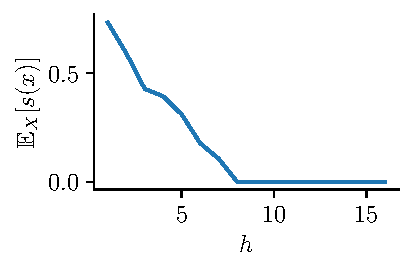
\includegraphics[scale=0.85]{data/chapter_intro/ae_reconstruction}\caption{The figure demonstrates the ability of an autoencoder to reconstruct
data. The dimensionality of the latent space $\mathcal{Z}$ is on
the x--axis, while the average reconstruction error over the whole
dataset is on the y--axis. Note that although the artificial dataset
is 16--dimensional, it only contains 8 non--correlated dimensions
while the remaining are a linear combination of them. This results
in the error dropping to zero for $\text{dim}(\mathcal{Z})>=8$ where
the model is able to disentangle the correlations and learn the identity
function.}
\label{fig:ae_reconstruction}
\par\end{centering}
\end{figure}

Suppose that $p(x)$ is the distribution of the normal data in $\mathcal{X}$
space. After training with enough examples sampled from $p(x)$, an
autoencoder should be able to reconstruct any sample from $p(x)$
almost exactly with the average error given by the constraints of
the hidden layers, as demonstrated in \ref{fig:ae_reconstruction}.
In other words, the autoencoder has learnt the shape of the distribution.
When presented with a novel sample, the ability of the autoencoder
to reconstruct it might be used to decide whether the sample comes
from $p(x)$ or not. Indeed, the most naive way of using autoencoders
for anomaly detection is assuming that $p(x)$ is the distribution
of normal data and training them using normal samples. Then, for a
novel sample $x$ the reconstruction error of the trained network
($\bar{\phi}$ and $\bar{\theta}$ are the learnt parameters of the
autoencoder)

\begin{equation}
f_{AE}(x)=\mathcal{L}_{r}(x,\bar{\phi},\bar{\theta})\label{eq:ae_score}
\end{equation}
can be used as a an anomaly score function with the assumption that
an anomaly is going to produce a larger reconstruction error due to
not coming from $p(x)$.


\subsection{Ensemble-based}

MOGAAL

\subsection{Hybrid - two-stage models}

\subsection{self-supervised methods}

\section{Anomaly detection datasets}
